\documentclass{notes}
\author{Ritchie Cai, Matthew Mosley \& Corey Higgins}
\title{Inverted Pendulumn Modeling}

\begin{document}
\maketitle 

\section{Description}
Our design project is to simulate and implement a inverted pendulum using 
$\text{Lego Mindstorm EV3}^{\textregistered}$. 

\section{Physical Model}

The rod on top of the cart can only lean forward and backward. 
Base cart also can move only move back and forth. 
When the rod is out of balance and leaning toward one side, the cart will accelerate toward the same
direction to make sure the rod is back to resting position relative to the cart.

\begin{figure}[!h]
  \begin{center}
    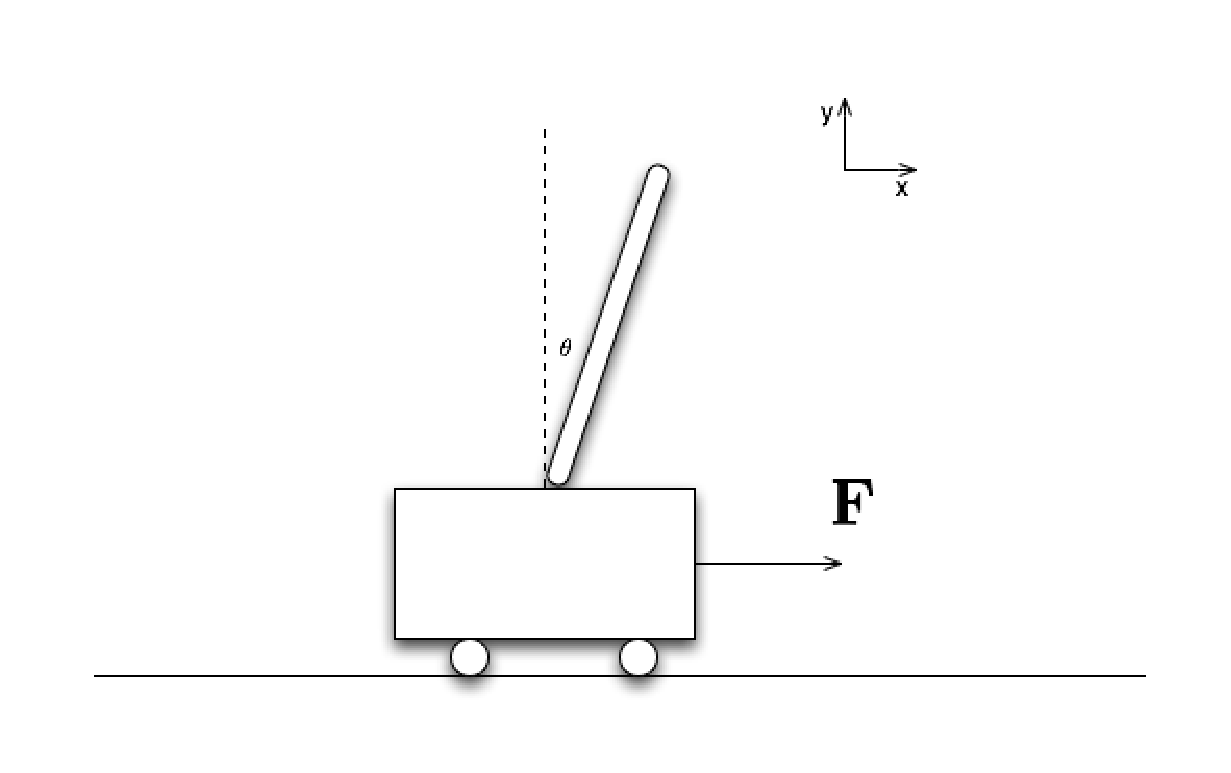
\includegraphics[width=3.5in]{pics/full_system.eps}
  \end{center}
  \caption{System setup for inverted pendulum}
  \label{fig:full_system}
\end{figure}


\section{Mathematical Model}



\subsection{X-axis}
One the horizontal, x-axis, we have:

\begin{align*}
  F_x & = F_{cart} + F_{rod} \\
  F_{cart} & = M\ddot{x}  \\
  F_{rod}  & = m a_x + m a_{p} \\
          & = m \ddot{x} + m (a_{t} + a_{c})
\end{align*}

where $a_x$, $a_t$ and $a_c$ are acceleration of x-axis, tangential and centripical respectively. 

\begin{figure}[!h]
  \begin{center}
    \begin{minipage}[b]{3.5in}
      \centerline{\mbox{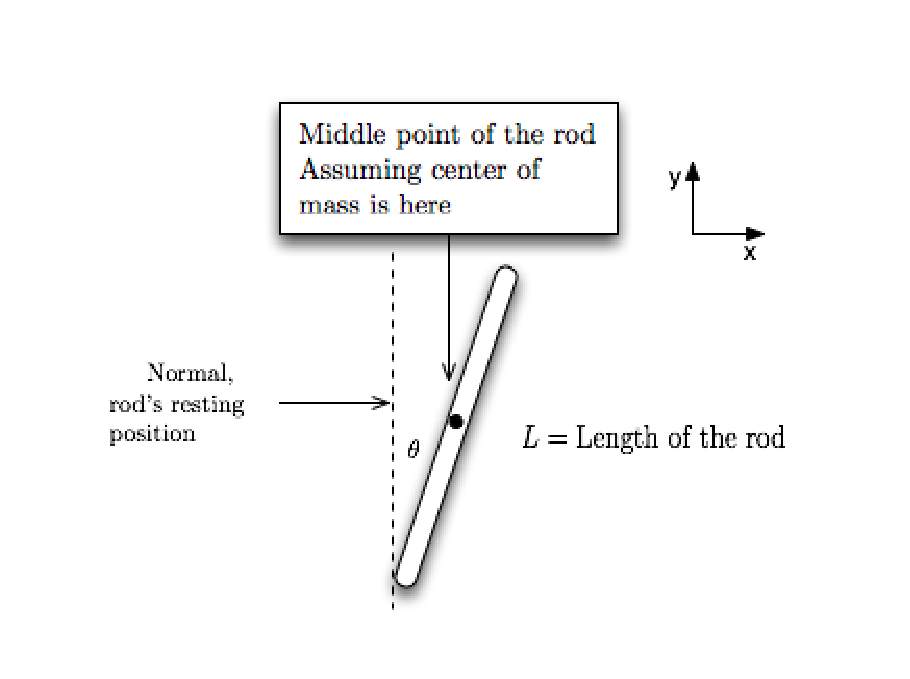
\includegraphics[width=3.5in]{pics/rod.eps}}}
    \end{minipage}
    \begin{minipage}[b]{3.5in}
      \centerline{\mbox{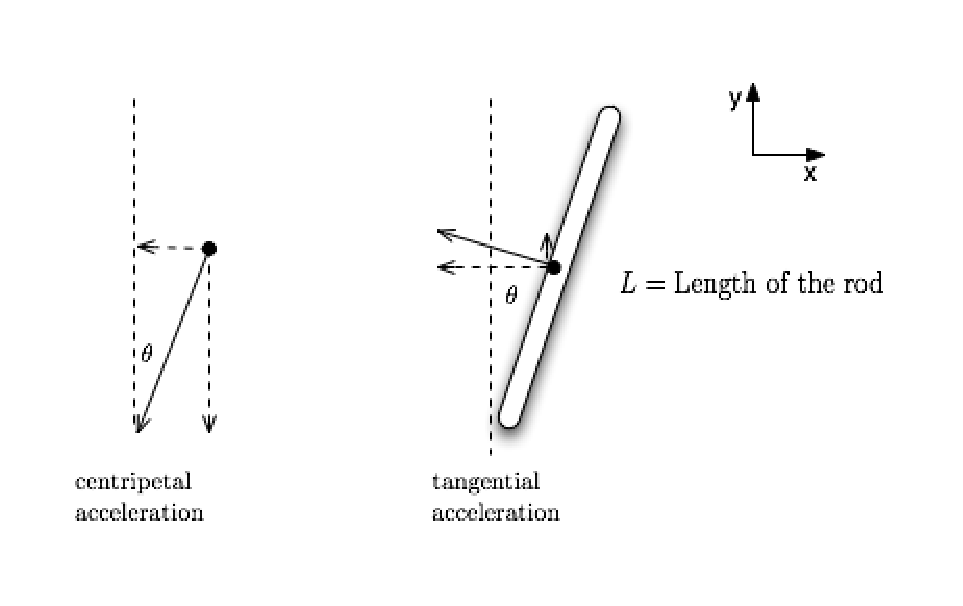
\includegraphics[width=3.5in]{pics/rod_acceleration.eps}}}
    \end{minipage}
    
  \end{center}
  \caption{Angular acceleration disection for the rod}
  \label{fig:angular_rod}
\end{figure}

According to figure~\ref{fig:angular_rod}, angular accelerations for the rod on x-axis can be
expressed as:
\begin{align*}
  a_t & = -\dfrac{L}{2} \ddot{\theta} \\
  a_c & = -\dfrac{L}{2} \dot{\theta}^2
\end{align*}

Since we are only interested in the components on the x-axis, we have:

\begin{align*}
  a_t & = -\dfrac{L}{2} \ddot{\theta} \cos \theta \\
  a_c & = -\dfrac{L}{2} \dot{\theta}^2 \sin \theta
\end{align*}

So 

\begin{align*}
  F_{rod} & = m \ddot{x} + m (a_{t} + a_{c}) \\
         & = m \ddot{x} -m\dfrac{L}{2} \ddot{\theta} \cos \theta 
                        -m\dfrac{L}{2} \dot{\theta}^2 \sin \theta \\
  F_x & = F_{cart} + F_{rod} \\
      & = M\ddot{x} + m \ddot{x} - m\dfrac{L}{2} \ddot{\theta} \cos \theta 
                    - m \dfrac{L}{2} \dot{\theta}^2 \sin \theta \\
      & = (M + m) \ddot{x} - m\dfrac{L}{2} \ddot{\theta} \cos \theta 
                    - m \dfrac{L}{2} \dot{\theta}^2 \sin \theta
\end{align*}
\FloatBarrier


\subsection{Y-axis}
Using Newton's second law for the vertical motion of the pendulum gives

\begin{align}
  F_y - mg & = m\frac{d^2y_G}{dt^2}\label{eqn:eq1}
 \end{align}
 
 Since $ y_G = l/2\cos(\theta)$,

 \begin{align}
   \frac{dy_G}{dt} & = \frac{d(l/2\cos\theta)}{dt} = -l/2\sin\theta\frac{d\theta}{dt} \nonumber\\
   \frac{d^2y_G}{dt^2} & = \frac{d}{dt}\left(-l/2/2 \sin\theta \frac{d\theta}{dt}\right) \nonumber\\
   & = -l/2/2\left(\frac{d\sin\theta}{dt}\frac{d\theta}{dt} + \sin\theta\frac{d^2\theta}{dt^2}\right) \nonumber\\
   & = -l/2\left( \cos\theta \left(\frac{d\theta}{dt}\right)^2 + \sin\theta\frac{d^2\theta}{dt^2}   \right) \nonumber\\
   & = -l/2\cos\theta\left(\frac{d\theta}{dt}\right)^2-l/2\sin\theta\frac{d^2\theta}{dt^2}\label{eqn:eq2}
 \end{align}
 
 Using Equation~\ref{eqn:eq2}, Equation~\ref{eqn:eq1} can be written as 
 \begin{align*}
   F_y - mg & = m\left(-l/2\cos\theta\left(\frac{d\theta}{dt}\right) - l/2\sin\theta\frac{d^2\theta}{dt^2}\right)
 \end{align*}
 
 Thus, the vertical reaction force, $F_y$, can be written as
 \begin{align*}
   F_y & = mg + m\left(-l/2\cos\theta\left(\frac{d\theta}{dt}\right) - l/2\sin\theta\frac{d^2\theta}{dt^2}\right)
 \end{align*}
 
 For any object, the relationship between the moment applied on an object and its angular acceleration is given by the following relationship
 \begin{align}
   \sum \overline{M} = I\frac{d^2\theta}{dt^2}\label{eqn:eq3}
 \end{align}
 
 where $\overline{M}$ is the moment due to a given force and defined as 
 
 \begin{align*}
   \overline{M} = \vec{F} \times \vec{r}
 \end{align*}
 
 where $\vec{F}$ is the force vector, $\vec{r}$ is the position vector of the object with respect to the point about which the moments are being summed, and $I$ is the angular momentum of the object. For the pendulum, summing the moment around the center of gravity, Equation~\ref{eqn:eq3} can be written as


\end{document}
